\chapter{Le système international d'unité (SI)}
\label{chap:si}

Le \textbf{Système international d'unités (abrégé SI)}, basé sur le \textbf{système métrique}, est le système d'unités le plus largement employé du monde. Il s'agit d'un système d'unités décimal (on passe d'une unité à ses multiples ou sous-multiples à l'aide de puissances de 10). C'est la Conférence générale des Poids et mesures (CGPM), rassemblant des délégués des états membres de la Convention du Mètre, qui décide de son évolution, tous les quatre ans, à Paris.

L'abréviation de \textless\textless\ Système international\ \textgreater\textgreater est SI, \textbf{quelle que soit la langue utilisée}\footnote{oui, \textit{même} en anglais}. La norme internationale ISO 1000 (ICS 01 060) décrit les unités SI et les recommandations pour l'emploi de leurs multiples et de certaines autres unités.

\section{Les sept unités de base SI}

\subsection{Origine}

Le nombre minimal d'unités possibles est basé sur le nombre minimal de grandeurs indépendantes et fondamentales permettant de décrire les lois de l'Univers. On comprendra aisément que l'\textbf{espace}, le \textbf{temps} et la \textbf{masse} sont des grandeurs ne pouvant pas s'exprimer les unes en fonction des autres, et que ces trois grandeurs définissent forcément \textbf{les trois premières unités fondamentales} de tout système métrologique, qui sont respectivement, en unités SI, le mètre, la seconde, le kilogramme.

Il existe une quatrième grandeur fondamentale, la \textbf{charge électrique}, irréductible aux  précédentes: on ne peut pas traduire la charge de l'électron ou du proton en une combinaison de masse, distance, et/ou temps~! A noter que c'est l'unité du courant électrique, soit la quantité de charge électrique qui passe dans un conducteur par unité de temps, qui constitue la quatrième unité fondamentale - l'ampère (A) - et non l'unité de la charge, le coulomb (C).

Pour continuer, il existe encore d'autres grandeurs fondamentales dont on ne parle presque jamais en dehors du monde de la physique subatomique: les charges liées aux interactions entre les particules fondamentales constitutives des protons et neutrons (les quarks), ainsi qu'entre les électrons et leur différentes versions (positron, muon etc.) Ces deux interactions se nomment l'interaction forte (pour les quarks) et faible (pour les électrons), mais ont une portée se limitant essentiellement aux dimensions du noyau de l'atome, et leurs effets ne se font ressentir que lors des expériences de physique des particules.

De la même manière que la charge électrique est le véhicule de la force électromagnétique, il existe des charges véhiculant les interactions forte et faible (nous ne les décrirons pas ici). Or, ces charges ne sont pas exprimables en termes des 4 unités fondamentales précédentes, elles constituent par conséquent de nouvelles grandeurs indépendantes, pour lesquelles des unités sont définies. Ceci dit, étant donné que ces charges n'ont d'importance que dans le domaine spécialisé de la physique des particules, et qu'elles sont loin d'avoir des applications courantes dans le monde actuel (hormis dans le domaine de l'imagerie médicale nucléaire), ces unités ne sont pas (encore) incluses comme unités fondamentales SI.

Aux quatre unités fondamentales ci-dessus, le système SI ajoute trois autres unités, le \textbf{kelvin} pour la température, la \textbf{candela} pour les mesures photométriques (quantité de lumière) et la \textbf{mole}, pour la quantité de matière.

Formellement, le kelvin et la candela ne sont pas des unités fondamentales: la température est en fait une mesure de l'énergie d'agitation thermique (oscillation, vitesse) des particules constituantes d'un corps à une température donnée; un flux de lumière n'est rien d'autre qu'un flux de photons véhiculant une certaine énergie. Or, l'énergie est exprimable en termes de distance, de masse et de temps.

La mole est en revanche une unité assez particulière, puisqu'elle ne correspond à aucune grandeur fondamentale des lois de la physique, au contraire des unités ci-dessus. Elle trouve son origine en chimie, où l'on a trouvé bien plus pratique, pour désigner un nombre d'atomes ou de molécules au sein d'une solution, de les regrouper par rapport à un nombre de bases, très grand, le nombre d'Avogadro, égal à $6.022141293\times 10^{23}$, typique du nombre d'atomes/molécules que l'on trouve dans les préparations de chimie\footnote{on consultera avec intérêt la page Wikipédia dédiée à ce sujet}. Il est en effet par exemple plus simple d'indiquer qu'il y a 3.5 moles d'une certaine molécule dans une solution donnée que de dire qu'il y en a $21.08\times 10^{23}$.

\subsection{Définitions}

Considérons l'unité de distance fondamentale, le mètre. Afin que cette référence soit disponible partout dans le monde, nous pourrions par exemple reproduire le mètre étalon conservé au \textbf{Bureau international des Poids et mesures (BIPM)} à Sèvres, France. Cette procédure présente cependant deux inconvénients majeurs : (1) tout procédé de reproduction ne saurait être exempt d'erreurs, (2) il faut avoir accès au mètre étalon.

Pour pallier à ces inconvénients, il a été décidé de définir le mètre non plus par rapport à un étalon physique, un objet bien réel, mais d'utiliser une propriété fondamentale de la matière, indépendante du temps et de l'espace, c'est-à-dire disponible partout et tout le temps, et parfaitement invariable, ou constante. On a donc choisi de définir le mètre comme la distance parcourue par la lumière, dans le vide, durant $1/299'792'458$ secondes exactement. Tout laboratoire bien équipé pourra reproduire cette expérience, et donc définir avec toute la précision requise une distance, entre deux plans de référence bien accessibles, égale au mètre ou à un de ses multiples ou sous-multiples.

L'exemple du mètre décrit le principe que l'on applique aujourd'hui à la définition des unités fondamentales SI. Seul le kilogramme est encore défini par rapport à un objet matériel concret – une masse composée d'un alliage de platine et d'iridium conservé au BIPM - susceptible de s'altérer. Des recherches ont d'ailleurs actuellement lieu pour remplacer cette définition par une autre, utilisant cette fois un phénomène physique, inaltérable par nature.

\newpage

\begin{center}
\begin{tabular}[t]{>{\pbs\raggedright}p{2.5cm}
                   >{\pbs\centering}p{2.2cm}
                   >{\pbs\centering}p{2.3cm}
                   >{\pbs\raggedright}p{7cm}}
\hline\hline
\textbf{Grandeur} & \textbf{Nom} & \textbf{Symbole SI} & \textbf{Définition, remarques}\\
\hline
longueur & mètre & m &
Le mètre est la longueur du trajet parcouru dans le vide par la lumière pendant 1/299'792'458 secondes. Historiquement, la première définition officielle du mètre (1791) était basée sur la circonférence de la terre, et valait 1/40'000'000 du périmètre de notre planète.
\\ \hline
masse & kilogramme & kg &
Le kilogramme est la masse d'un cylindre composé d'un alliage de platine (90 \%) et d'iridium (10\%), conservé au Bureau international des Poids et mesures. Historiquement, la définition du kilogramme était la masse d'un décimètre cube d'eau.
\\ \hline
temps & seconde & s &
La seconde est la durée de temps associée à 9'192'631'770 oscillations de l'onde électromagnétique (photons) émise lors de la transition des électrons entre les deux sous-niveaux d'énergie de l'état d'énergie fondamental de l'atome de césium 133 ($^{133}$Cs) à la température de 0 kelvin. La seconde était à l'origine basée sur la durée (instable) du jour terrestre, d'une durée de 86'400 secondes.
\\ \hline
\end{tabular}
\end{center}
\begin{center}
\begin{tabular}[t]{>{\pbs\raggedright}p{2.5cm}
                    >{\pbs\centering}p{2.2cm}
                    >{\pbs\centering}p{2.3cm}
                    >{\pbs\raggedright}p{7cm}}
\hline
courant électrique & ampère & A &
L'ampère est l'intensité d'un courant constant qui, maintenu dans deux conducteurs parallèles, rectilignes, de longueur infinie, de section circulaire négligeable et placés à une distance de un mètre l'un de l'autre dans le vide produirait entre ces conducteurs une force égale à $2\times10^{-7}$ newton par mètre de longueur.
\\ \hline
température & kelvin & K	&
Le kelvin, unité de température thermodynamique, est la fraction 1/273.16 de la température thermodynamique du point triple de l'eau. Le point triple de l'eau est, dans le diagramme pression-température, un point où l'eau peut exister dans les trois états, soit solide, liquide et gazeux. La température associée à cet état est de 273.16 K. A noter que l'on écrit K et non $^{\circ}$K.
\\ \hline
quantité de matière & mole & mol	&
La mole est la quantité de matière d'un système contenant autant d'entités élémentaires qu'il y a d'atomes dans 0.012 kg de carbone 12 ($^{12}$C). Ce nombre d'entités élémentaires est appelé nombre d'Avogadro, et vaut $\mathcal{N}_{A}=6.02214129(27)\times10^{23}\,\text{mol}^{-1}$. Lorsque l'on emploie la mole, les entités élémentaires doivent être spécifiées et peuvent être des atomes, des molécules, des ions, des électrons, d'autres particules ou des groupements spécifiés de telles particules.
\\ \hline
\end{tabular}
\end{center}
\begin{center}
\begin{tabular}[t]{>{\pbs\raggedright}p{2.5cm}
                    >{\pbs\centering}p{2.2cm}
                    >{\pbs\centering}p{2.3cm}
                    >{\pbs\raggedright}p{7cm}}
\hline
intensité lumineuse & candela & cd &
La candela est l'intensité lumineuse, dans une direction donnée, d'une source qui émet un rayonnement monochromatique de fréquence $540\times10^{12}$ hertz et dont l'intensité énergétique dans cette direction est de 1/683 watt par stéradian.
\\ \hline\hline
\end{tabular}
\end{center}


\section{Unités dérivées}


Les unités dérivées font partie du système SI et sont déduites des sept unités de base.
\begin{center}
\begin{tabular}[t]{>{\pbs\raggedright}p{28mm}
                    >{\pbs\centering}p{15mm}
                    >{\pbs\centering}p{12mm}
                    >{\pbs\centering}p{22mm}
                    >{\pbs\centering}p{22mm}
                    >{\pbs\raggedright}p{32mm}}
\hline\hline
\textbf{Grandeur} & \textbf{Nom} & \textbf{Sym. SI} & \textbf{lien avec autres unités} & \textbf{lien avec unités de base} & \textbf{Relation physique}\\
\hline
Fréquence & hertz & Hz & --- & 1/s & Fréquence = 1/période \\ \hline
Force & newton & N & --- & kg m/s$^2$ & Force = masse $\times$ accélération \\ \hline
Contrainte, pression & pascal & Pa	& N/m$^2$ & kg/m/s$^2$ & Pression = force / surface \\ \hline
Energie, travail, quantité de chaleur & joule & J & N m & kg m$^2$/s$^2$	& Travail = force$\times$distance;
énergie cinétique = masse$\times$vitesse$^2$/2 \\ \hline
Puissance, flux énergétique et flux thermique & watt & W & J/s & kg m$^2$/s$^3$ & Puissance = travail / temps \\ \hline
Charge électrique, quantité d'électricité & coulomb & C & --- & A s & Charge = courant$\times$temps \\ \hline
\end{tabular}
\end{center}

\begin{center}
\begin{tabular}[t]{>{\pbs\raggedright}p{28mm}
                    >{\pbs\centering}p{17mm}
                    >{\pbs\centering}p{11mm}
                    >{\pbs\centering}p{22mm}
                    >{\pbs\centering}p{22mm}
                    >{\pbs\raggedright}p{32mm}}
\hline
Force électromotrice, différence de potentiel (tension) & volt & V & J/C & kg m$^2$/s$^3$/A & Tension = travail / charge
\\ \hline
Résistance électrique & ohm & $\Omega$ & V/A & kg m$^2$/s$^3$/A$^2$ & Résistance =  tension / courant
\\ \hline
Conductance électrique & siemens & S	& A/V & s$^3$A$^2$/kg/m$^2$ & Conductance = courant / tension
\\ \hline
Capacité électrique & farad & F & C/V & s$^4$A$^2$/kg/m$^2$ & Capacité = charge / tension
\\ \hline
Induction magnétique & tesla & T	& V s/m$^2$ & kg/s$^2$/A & Induction = tension$\times$temps / surface
\\ \hline
Flux d'induction magnétique & weber & Wb	& V s & kg m$^2$/s$^2$/A & Flux d'induction = tension$\times$temps
\\ \hline
Inductance électrique & henry & H & V s/A & kg m$^2$/s$^2$/A$^2$ & Inductance = tension$\times$temps / courant
\\ \hline
Température & degré Celsius & $^{\circ}$C & --- & K & T [$^{\circ}$C]=T [K]-273.15
\\ \hline
Flux lumineux & lumen & lm & --- & cd sr & ---
\\ \hline
Éclairement lumineux & lux & lx & --- & cd sr/m$^2$ & ---
\\ \hline
Nombre de désintégrations par seconde (radioactivité) & becquerel & Bq & --- & 1/s & ---
\\ \hline
Dose de radioactivité absorbée & gray & Gy & J/kg & m$^2$/s$^2$ & ---
\\ \hline
Équivalent de dose radioactivité absorbée & sievert & Sv & J/kg & m$^2$/s$^2$ & ---
\\ \hline
Activité catalytique & katal & kat & --- & mol/s & ---
\\ \hline\hline
\end{tabular}
\end{center}


\section{Préfixes du système SI}


Les préfixes du système international d'unités simplifient la manipulation des mesures qui ont des rapports élevés d'unité (par exemple de 0.1 cm à 1'000 m). Ces préfixes renvoient à des multiples et des fractions de 10 ou de 1000.  Les préfixes et noms correspondants sont donnés dans le tableau ci-après. On notera que les préfixes s'écrivent avec une lettre minuscule à partir et en dessous de l'échelle des milliers. \textbf{Il est fondamental d'observer très exactement ces conventions internationales}.

\begin{table}[htbp]
%\footnotesize
\begin{center}
\begin{tabular}{>{\pbs\raggedright}p{1cm}>{\pbs\raggedright}p{1.4cm}>{\pbs\centering}p{1.5cm}ll}
$10^n$ & Préfixe & Sym. SI & Nombre décimal & Échelle \\ \hline
$10^{24}$  & yotta &     Y & 1'000'000'000'000'000'000'000'000 & Quadrillion \\
$10^{21}$  & zetta &     Z & 1'000'000'000'000'000'000'000 & Trilliard \\
$10^{18}$  &   exa &     E & 1'000'000'000'000'000'000 & Trillion \\
$10^{15}$  &  péta &     P & 1'000'000'000'000'000 & Billiard \\
$10^{12}$  &  téra &     T & 1'000'000'000'000 & Billion \\
$10^{9}$   &  giga &     G & 1'000'000'000 & Milliard \\
$10^{6}$   &  méga &     M & 1'000'000 & Million \\
$10^{3}$   &  kilo &     k & 1'000 & Millier \\
$10^{2}$   & hecto &     h & 100 & Cent \\
$10^{1}$   &  déca &    da & 10 & Dix \\
$10^{0}$   &   --  &    -- & 1 & Unité \\
$10^{-1}$  &  déci &     d & 0.1	& Dixième \\
$10^{-2}$  & centi &     c & 0.01 & Centième \\
$10^{-3}$  & milli &     m & 0.001 & Millième \\
$10^{-6}$  & micro & $\mu$ & 0.000'001 & Millionième \\
$10^{-9}$  &  nano &     n & 0.000'000'001 & Milliardième \\
$10^{-12	}$ &  pico &     p & 0.000'000'000'001 & Billionième \\
$10^{-15	}$ & femto &     f & 0.000'000'000'000'001 & Billiardième \\
$10^{-18	}$ &  atto &     a & 0.000'000'000'000'000'001 & Trillionième \\
$10^{-21	}$ & zepto &     z & 0.000'000'000'000'000'000'001 & Trilliardième \\
$10^{-24	}$ & yocto &     y & 0.000'000'000'000'000'000'000'001 & Quadrillionième \\ \hline
\end{tabular}
\end{center}
\end{table}

\newpage

\section{Unités angulaires}

\begin{wrapfigure}[20]{l}[0pt]{5cm}
   \centering
   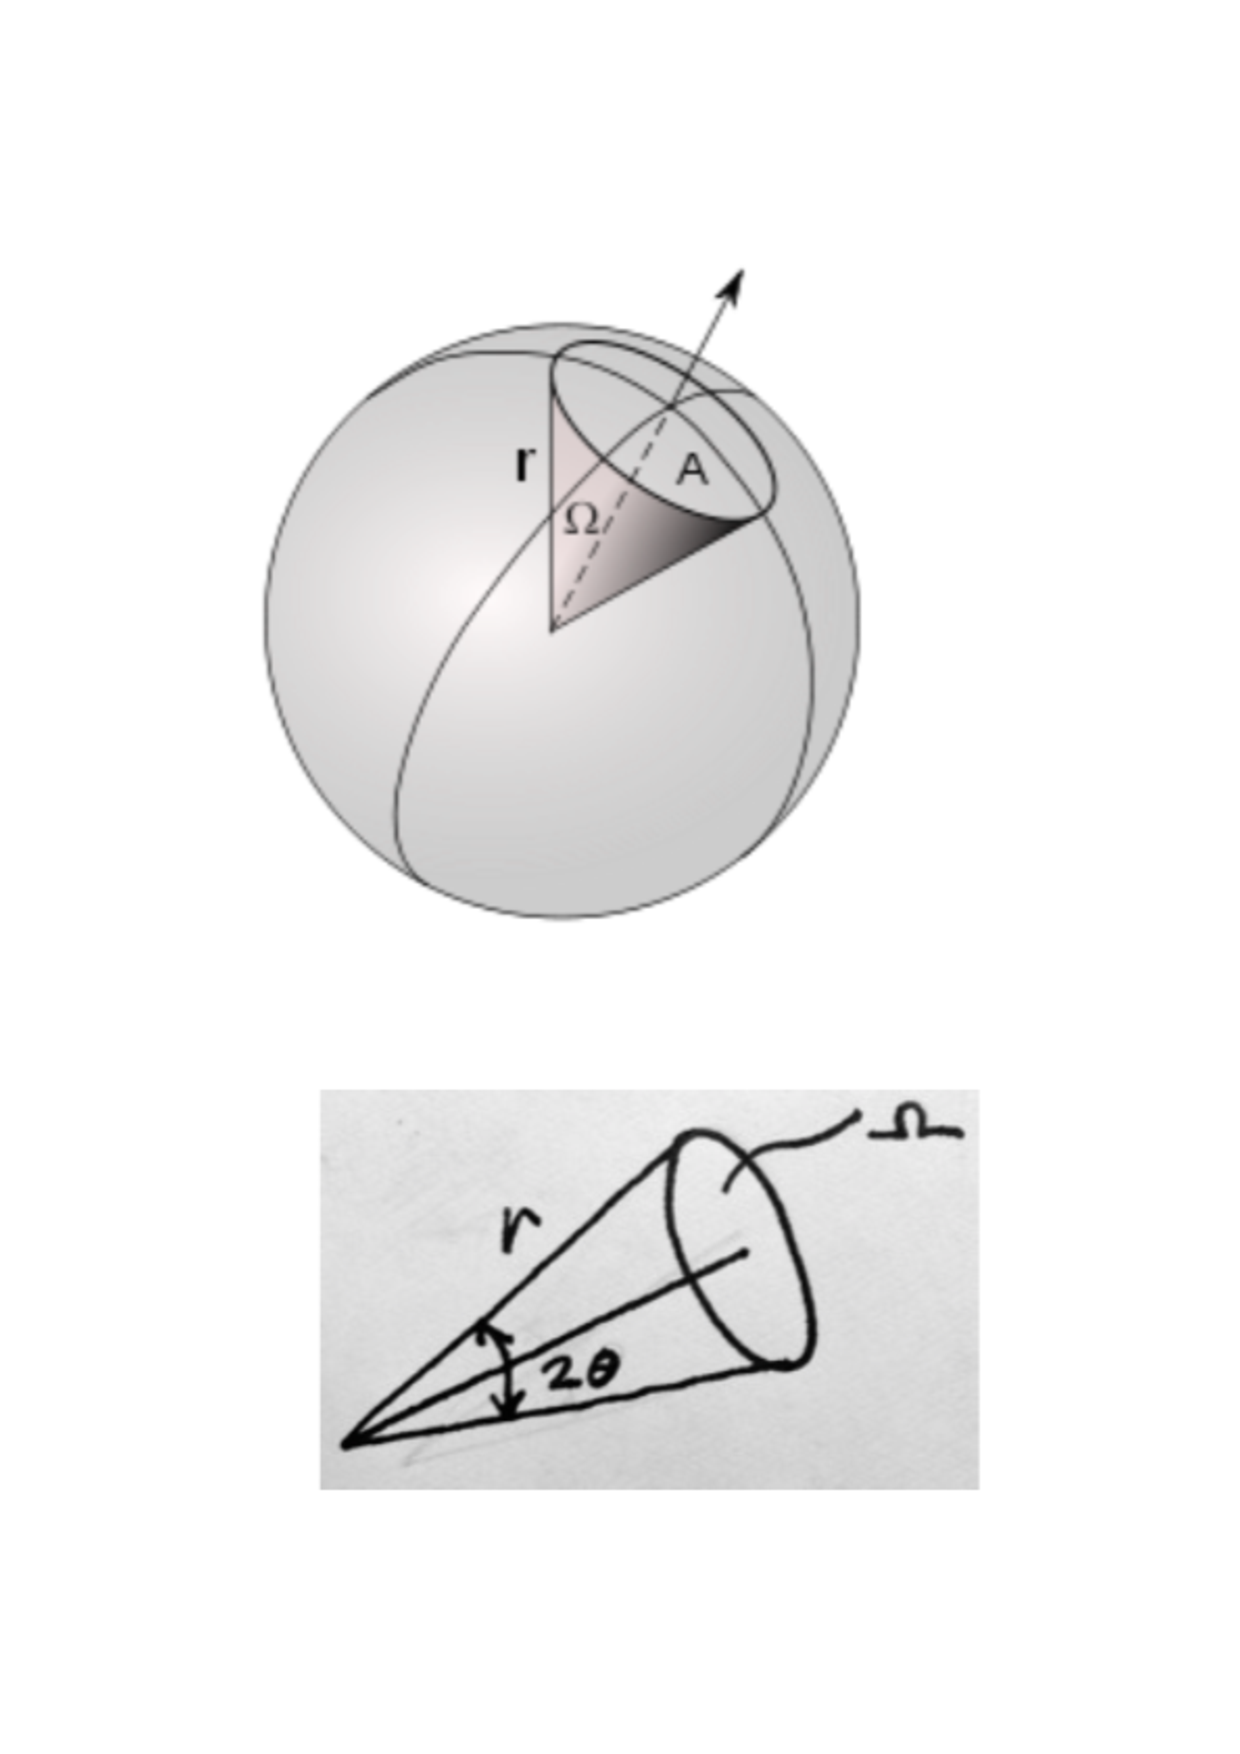
\includegraphics[width=5cm]{assets/figures/defAngleSolide.pdf}
   \caption{Définition de l'angle solide.}
   \label{fig:angles}
\end{wrapfigure}
À côté des unités de base et des unités dérivées, il existe deux unités angulaires:

\paragraph{L'unité d'angle plan: le radian (symbole: rad)} Soit un secteur de cercle de rayon $r$ et de longueur d'arc $l$. L'angle $\theta$ associé au secteur, en radian, est défini par le rapport
$$
\theta=\frac{l}{r}\ \ [\text{rad}]
$$
180$^\circ$ correspondant à $\pi$ rad, on a que 1 rad $\approx$ 57.3$^\circ$.

\paragraph{L'unité d'angle solide: le stéradian (symbole: sr)} Soit un cône dont l'angle au sommet est de $2\theta$ [rad], et soit $A$ l'aire de la calotte sphérique formée par l'intersection du cône avec la surface de la sphère de rayon $r$ (figure~\ref{fig:angles}). L'angle solide $\Omega$ associé au cône est défini par le rapport
$$
\Omega=\frac{A}{r^2}\ \ [\text{sr}]
$$
L'aire d'une sphère de rayon $r$ étant donnée par $4\pi\,r^2$, on trouve que l'angle solide de la sphère est égal à $4\pi$ sr, et de la demi-sphère $2\pi$. On peut aussi montrer que
$$
\Omega=2\pi(1-\cos\theta)
$$

Les grandeurs \textless\textless\ angle plan \ \textgreater\textgreater et \textless\textless\ angle solide \ \textgreater\textgreater sont des unités sans dimension - puisqu'il s'agit de rapport de longueurs et de surface - qui peuvent être indiquées ou non dans les expressions des unités dérivées.

\section{Règles d'écriture des unités et symboles SI}

\begin{itemize}

\item le nom de l'unité est un nom commun même pour les unités provenant de noms propres : volt, ampère, kelvin, tesla etc;
\item les symboles SI des unités sont écrits en police droite, et en minuscules, \textbf{sauf} si le nom de l'unité est dérivée d'un nom propre: dans ce cas la première lettre du symbole est en majuscule, par exemple N (Newton), J (Joule), V (Volta), Bq (Bequerel);
\item les symboles SI sont invariables au pluriel;
\item les symboles SI sont écrits sans point final;
\item les symboles SI doivent être placés après les valeurs numériques, en laissant un espace entre valeur et symbole, donc 30 m est juste, 30m ne l'est pas;
\item le produit de 2 unités est indiqué par un point, qui peut être omis si aucune confusion n'est possible, par exemple 1 mN est un millinewton et non un mètre-newton (c.-à-d. un joule), sinon nous aurions écrit m$\cdot$N !
\item le quotient est indiqué par une barre oblique, ou alors on peut utiliser les puissances négatives, comme avec m/s$^2$ ou m$\cdot$s$^{-2}$, mais pas ms$^{-2}$ car alors ms peut être interprété comme indiquant des millisecondes;
\item lorsque l'unité suit une valeur numérique, on ne met \textbf{jamais} de crochets autour de l'unité; on ne place l'unité entre crochets que dans les formules, par exemple la fameuse formule d'Einstein s'écrira
$$
E=mc^2\ \text{[J]}\ \ \ \ \text{mais par contre}\ \ \ \ E=10^6\ \text{J}
$$
\end{itemize}
Quelques exemples d'écriture  fausses et justes:

\begin{center}
\begin{tabular}{lll}
faux & juste & interprétation\\\hline
$99Kg$& 99 kg & 99 kilogramme\\
$25 [ms]$ & 25 ms & 25 milliseconde\\
$12 \mu v$ & 12 $\mu$V & 12 microvolt\\
100 K*m & 100 K$\cdot$m & 100 kelvin$\cdot$mètre\\\hline
\end{tabular}
\end{center}